\chapter{分子演化与系统基因组学}\label{ch:b3:molecular-evolution}

1968 年，木村资生做了一次计算，令该领域为之震动。
他比较了共同祖先已由化石定年的哺乳动物的血红蛋白、细胞色素及其他蛋白质，
发现氨基酸以约每个位点每十亿年一次的速率被替换，
若就整个哺乳动物基因组和每一代来计算，
则大约每两年就有一个新替换在种群中固定下来。
霍尔丹十年前已指出，自然选择至多能固定大约
每三百代一个替换，若再快，
则因损失后代而付出的代价便无法承受。
这一算术只留下一条出路：
DNA 中积累的大多数变化并非由选择驱动，
而是中性的，在有限种群中由随机性固定，其
速率——如本章首个定理所示——恰好就是
突变速率。\omterm{thm:b3:molecular-evolution:neutral}{中性理论}成为分子演化的原假设，
即用以检测选择的基准；
\omterm{prop:b3:molecular-evolution:clock}{分子钟}则成为测定化石所无法定年者年代的一种方法；
而此后测序的基因组则提供了工具，使人们能够逐个基因
地看清选择在何处起了作用，新基因如何由旧基因产生，以及
为何一个基因的系统树未必与其物种的系统树一致。

\section{遗传漂变、突变与中性速率}

\begin{theorem}[中性替换速率]\label{thm:b3:molecular-evolution:neutral}
\index{中性理论}\index{替换速率}\index{固定概率}\index{遗传漂变}
在含 $N$ 个个体的二倍体种群中，一个新突变
对适合度无影响，则其最终取代所有其他等位基因的概率为 $1/2N$，
（\emph{固定}），而被丢失的概率为 $1 - 1/2N$。若
$2N$ 个基因拷贝中的每一个以每代 $\mu$ 的速率突变，则每代
产生 $2N\mu$ 个新的中性突变，并且从长期来看，
替换积累的速率为
\[
k = 2N\mu\times\frac{1}{2N} = \mu :
\]
中性\emph{\omterm{thm:b3:molecular-evolution:neutral}{替换速率}}等于突变速率，
与种群大小无关。注定被固定的突变平均需要
$4N$ 代才能完成固定，因此大种群在途中保留的变异更多，
但固定速度并不因此加快。对于
选择优势为 $s$ 的突变，木村公式给出的\omterm{thm:b3:molecular-evolution:neutral}{固定
概率}为
\[
P(s) = \frac{1 - \mathrm{e}^{-2s}}{1 - \mathrm{e}^{-4Ns}} \approx 2s
\quad (4Ns \gg 1),
\]
因此选择优势为 \qty{1}{\%} 的突变，其\omterm{thm:b3:molecular-evolution:neutral}{固定概率}约为
\qty{2}{\%}——是中性突变在两千个个体种群中机会的四十倍，
但仍有五十次中四十九次被丢失；
而对于 $s < 0$ 且 $4N|s| \gg 1$ 的不利突变，几乎从不被固定，
而 $4N|s| \ll 1$ 者则表现为中性：选择
只能看到漂变无法掩盖的部分，分界为 $|s| \sim
1/4N$——\emph{近中性}。
\end{theorem}
\begin{proof}
中性：今天存在的某个拷贝将是遥远未来整个种群的祖先，
由对称性，$2N$ 个拷贝中的每一个成为祖先的可能性相同，
而新突变体只是一个拷贝，故其概率为
$1/2N$。速率：每代替换数 $=$（每代产生的突变数
）$\times$（每个突变被固定的概率）$= 2N\mu/2N$。木村公式
由描述漂变与选择下等位基因频率变化的扩散近似得出，
此处不加证明地承认；其极限
情形可直接检验：当 $s \to 0$ 时，$(2s)/(4Ns) = 1/2N$，即中性
值；对于 $4Ns \gg 1$，分母为 $1$，分子
$\approx 2s$。固定时间：中性等位基因的频率
以每代方差 $p(1-p)/2N$ 做随机游走，并且
到达 $1$ 的期望时间（以此为条件，起点为 $1/2N$）
为 $4N$ 代（木村与太田，1969），此处承认。
\end{proof}

\begin{omfigure}
\begin{tikzpicture}
\begin{semilogyaxis}[
  width=0.62\linewidth, height=5.6cm,
  axis x line=bottom, axis y line=left,
  xmin=-4, xmax=8, ymin=0.00002, ymax=0.2,
  xlabel={$4Ns$（标度选择系数）}, ylabel={固定概率},
  xlabel style={font=\small, at={(axis description cs:0.5,-0.12)}, anchor=north}, ylabel style={font=\small},
  tick label style={font=\small}, xtick={-4,-2,0,2,4,6,8}, ytick={0.0001,0.001,0.01,0.1}, yticklabels={$10^{-4}$,$10^{-3}$,$10^{-2}$,$10^{-1}$},
  clip=false,
]
\addplot[very thick, omDef, domain=-4:-0.05, samples=60] {(x/2000)/(1-exp(-x))};
\addplot[very thick, omDef, domain=0.05:8, samples=80] {(x/2000)/(1-exp(-x))};
\draw[dashed, gray] (axis cs:-4,0.0005) -- (axis cs:8,0.0005); \node[font=\scriptsize, gray, anchor=north west] at (axis cs:-3.9,0.00048) {中性，$1/2N$};
\addplot[thick, omThm, dashed, domain=1:8, samples=2] {2*x/(4*1000)};
\node[font=\scriptsize, omThm, anchor=north west] at (axis cs:5,0.0012) {$2s$ 渐近线};
\node[font=\scriptsize, omDef, anchor=south east, align=right] at (axis cs:-0.2,0.02) {近中性 \\当 $|4Ns| \lesssim 1$ 时};
\node[font=\scriptsize, omDef, anchor=south west] at (axis cs:-3.9,0.0008) {有害：几乎从不被固定};
\end{semilogyaxis}
\end{tikzpicture}

{\small 木村的\omterm{thm:b3:molecular-evolution:neutral}{固定概率}随标度
选择系数的变化（$N = 1000$）。在零附近，曲线经过
中性值；向右时趋近 $2s$ 上升，
向左则陡然下落。选择只作用于漂变无法掩盖的部分。}
\end{omfigure}

\begin{proof}[证据]
木村（1968）与金和朱克斯（1969）从速率出发作出论证：
所观察到的哺乳动物蛋白质间氨基酸\omterm{thm:b3:molecular-evolution:neutral}{替换速率}，
意味着每代替换数超过霍尔丹选择代价所允许的上限，
因此大多数替换必定是中性的。理论的预测
随后得到证实：速率在功能约束最少处最高——
同义位点、内含子、\omterm{def:b3:molecular-evolution:duplication}{假基因}以及密码子的第三位——
而在\omterm{def:b3:chromatin-epigenetics:nucleosome}{组蛋白}和泛素中最低，一亿年中仅改变
一个残基；物种内的变异水平随
突变与种群大小而变化；每年的\omterm{thm:b3:molecular-evolution:neutral}{替换速率}
在种群大小差异悬殊的谱系之间大致恒定，
这正是公式 $k = \mu$ 所要求的，而选择论的解释则不然。
其后的争论并未推翻这一理论：它确立了中性
速率作为衡量选择时的原假设。
\end{proof}

\begin{omfigure}
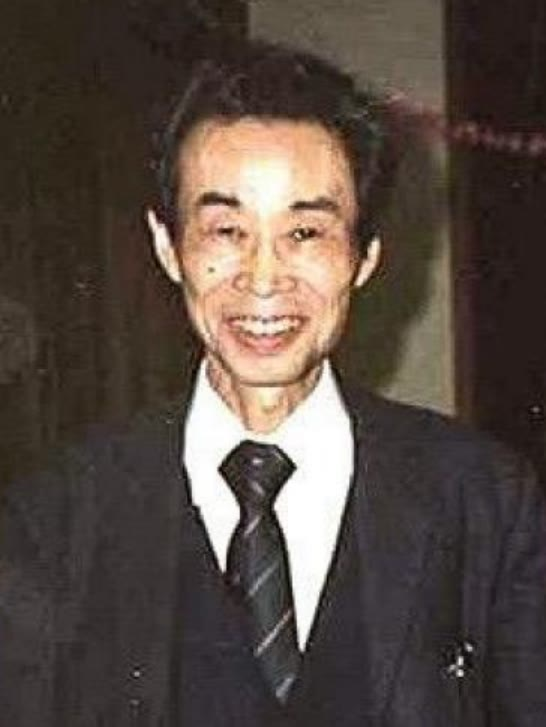
\includegraphics[width=0.34\linewidth]{images/book5/kimura.jpg}\hspace{0.05\linewidth}
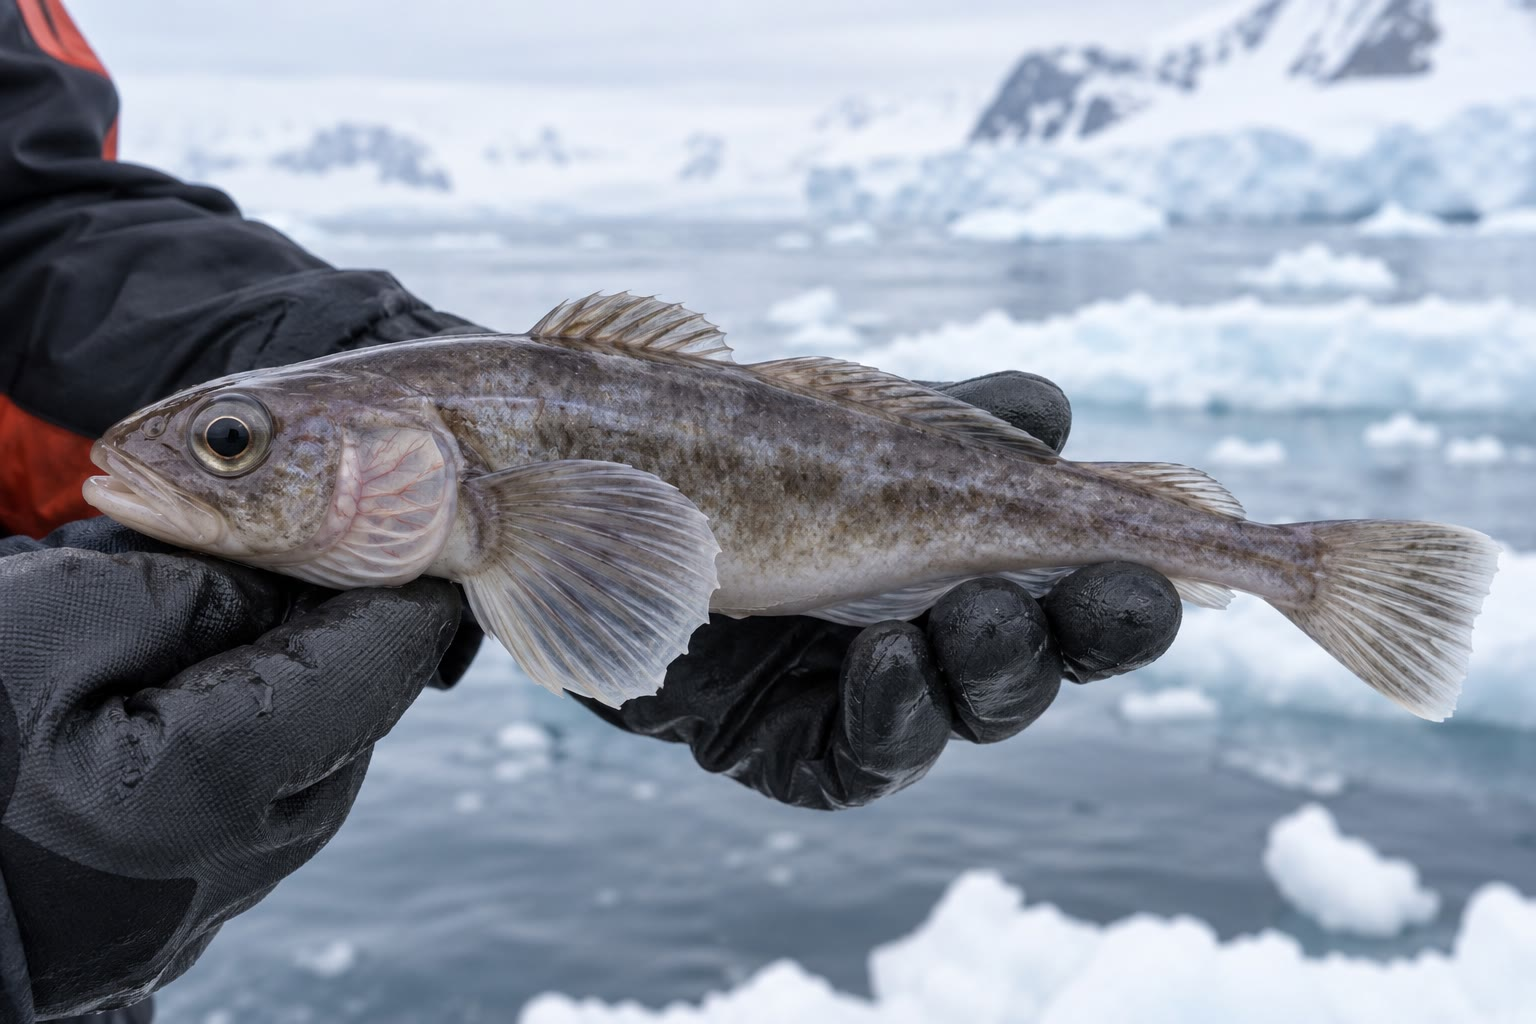
\includegraphics[width=0.5\linewidth]{images/book5/ai/b5-25-icefish.jpg}

{\small 左：木村资生（1924--1994），他证明了大多数分子水平的变化
是由偶然性固定的，其速率等于突变速率（照片，1986 年，CC BY 4.0）。右：
一种南极冰鱼，其血液借助一种抗冻糖蛋白免于凝固，该蛋白
约在一千万年前由一个重复的消化酶基因与
一段重复序列\omterm{def:b3:genomics:assembly}{组装}而成。}
\end{omfigure}

\section{分子钟}

\begin{proposition}[分子钟及其不规则性]\label{prop:b3:molecular-evolution:clock}
\index{分子钟}\index{校准}\index{速率异质性}\index{宽松分子钟}\index{世代时间效应}
若替换在两个谱系中以每位点每年恒定速率 $k$ 积累，
且这两个谱系于 $T$ 年前分化，则两者存在差异的位点比例在数值较小时为
$d \approx 2kT$：两条序列的散度即为一个
\emph{\omterm{prop:b3:molecular-evolution:clock}{分子钟}}（祖克坎德尔与鲍林，
1965），它可以由一个有化石定年的分化事件进行\emph{\omterm{prop:b3:molecular-evolution:clock}{校准}}，
此后即可用于读取没有化石的分化事件。\omterm{prop:b3:molecular-evolution:clock}{分子钟}具有随机性——它是一个泊松过程，
因此在固定位点数下 $d$ 的方差约等于其均值——
并且它以三种已知方式表现出不规则性。每种蛋白质
都有其自身的速率，由其中功能允许发生变化的位点比例决定：
纤维蛋白肽为 \num{8}，血红蛋白
为 \num{1}，细胞色素~$c$ 为 \num{0.3}，\omterm{def:b3:chromatin-epigenetics:nucleosome}{组蛋白}~H4 为 \num{0.01}，
单位为每位点每十亿年的替换数。谱系之间的速率也各不相同：由于
中性速率为每代 $\mu$，世代短的动物（啮齿类）每年积累的变化
比世代长的动物（灵长类、鲸类）更多——这就是
\emph{\omterm{prop:b3:molecular-evolution:clock}{世代时间效应}}，它被部分抵消了，
因为每代突变率随世代长度增加而升高。
此外，$d$ 会饱和：当许多位点已经发生变化后，
进一步的变化会落在已经变化过的位点上，因此原始差异必须校正多重打击，
正如\omterm{def:b3:bioinformatics:alignment}{比对}一章中的距离所做的那样。现代\emph{\omterm{prop:b3:molecular-evolution:clock}{宽松分子钟}}，
允许速率在统计模型中于各分支之间变化，并由许多化石同时\omterm{prop:b3:molecular-evolution:clock}{校准}；它们
给出人类与黑猩猩的分化时间为六至七百万年前，
有胎盘哺乳动物各目的分化接近白垩纪末，
动物与真菌的分化则在前寒武纪，
其不确定度为十至二十个百分点，
主要来源于化石。
\end{proposition}
\begin{proof}
两个谱系各自在每个位点积累 $kT$ 次替换，因此
在未被两次打击的位点上，二者之差为 $2kT$；
由一对有化石定年的物种可得 $k = d/2T$。泊松方差与
各蛋白质的速率由祖克坎德尔与鲍林、迪克森（1971）
以及木村资生对脊椎动物蛋白质集合的拟合得出；饱和校正
采用\omterm{def:b3:bioinformatics:alignment}{比对}一章中的朱克斯–康托尔公式，$d_{\text{校正}} =
-\tfrac{3}{4}\ln(1 - \tfrac{4}{3}p)$。谱系之间的速率差异
由相对速率检验证实：取外群 $O$ 与两个物种
$A$、$B$，在严格\omterm{prop:b3:molecular-evolution:clock}{分子钟}下 $d_{AO} - d_{BO}$ 应为零，
而啮齿类与灵长类之间的结果并非如此。
\end{proof}

\begin{omfigure}
\begin{tikzpicture}
\begin{axis}[
  width=0.68\linewidth, height=5.8cm,
  axis x line=bottom, axis y line=left,
  xmin=0, xmax=600, ymin=0, ymax=110,
  xlabel={分化以来的时间（百万年）}, ylabel={每 100 位点的替换数（校正后）},
  xlabel style={font=\small, at={(axis description cs:0.5,-0.12)}, anchor=north}, ylabel style={font=\small},
  tick label style={font=\small}, xtick={0,100,200,300,400,500,600}, ytick={0,20,40,60,80,100},
  clip=false,
]
\addplot[very thick, omThm, domain=0:130, samples=2] {2*0.4*x};
\addplot[very thick, omDef, domain=0:600, samples=2] {2*0.09*x};
\addplot[very thick, omMeth!70!black, domain=0:600, samples=2] {2*0.03*x};
\addplot[very thick, omProp!80!black, domain=0:600, samples=2] {2*0.001*x};
\addplot[only marks, mark=*, mark size=1.8pt, omDef] coordinates {(80,13) (100,20) (300,52) (400,75) (450,80)};
\addplot[only marks, mark=*, mark size=1.8pt, omMeth!70!black] coordinates {(80,4) (300,17) (450,29) (550,33)};
\addplot[only marks, mark=*, mark size=1.8pt, omThm] coordinates {(30,22) (80,68) (100,80)};
\node[font=\scriptsize, omThm, anchor=west] at (axis cs:132,104) {纤维蛋白肽};
\node[font=\scriptsize, omDef, anchor=south east] at (axis cs:600,108) {血红蛋白};
\node[font=\scriptsize, omMeth!70!black, anchor=north west] at (axis cs:530,35) {细胞色素 $c$};
\node[font=\scriptsize, omProp!80!black, anchor=south east] at (axis cs:600,1.5) {组蛋白 H4};
\end{axis}
\end{tikzpicture}

{\small \omterm{prop:b3:molecular-evolution:clock}{分子钟}，逐个蛋白质来看。每种蛋白质都以其自身的速率推进，
该速率由分子中功能允许自由变化的部分多少决定：纤维蛋白肽
在血液凝固时被切除并丢弃，其变化速度
比包装 DNA 的\omterm{def:b3:chromatin-epigenetics:nucleosome}{组蛋白}快数百倍。}
\end{omfigure}

\section{从序列中读取选择}

\begin{definition}[dN/dS]\label{def:b3:molecular-evolution:dnds}
\index{同义替换}\index{非同义替换}\index{dN/dS 比值}\index{纯化选择}\index{正选择}
在编码蛋白质的基因中，若一次替换不改变氨基酸，则称之为\emph{同义替换}，
若改变氨基酸，则称之为\emph{非同义替换}。由于遗传密码使大多数第三位
以及部分第一位的替换可以不改变氨基酸，
因此典型基因中约四分之一的可能突变为同义突变。
设 $d_{S}$ 为每个同义位点上的同义替换数，
$d_{N}$ 为每个非同义位点上的非同义替换数，
二者均经多重打击校正。同义替换接近中性，
因此 $d_{S}$ 估计的是 $2\mu T$——即\omterm{prop:b3:molecular-evolution:clock}{分子钟}；
而比值
\[
\omega = \frac{d_{N}}{d_{S}}
\]
该比值度量了选择对蛋白质所起的作用：若氨基酸变化与同义变化同样自由，
即无约束的情形（如\omterm{def:b3:molecular-evolution:duplication}{假基因}）时 $\omega = 1$；在\emph{纯化选择}下
$\omega < 1$，大多数变化被清除——典型基因的 $\omega \approx 0.1$ 至 $0.2$，
\omterm{def:b3:chromatin-epigenetics:nucleosome}{组蛋白}则为 $0.001$；在\emph{正选择}下 $\omega > 1$，
氨基酸变化的发生速度快于单靠漂变所能达到的速度——
例如 MHC 分子的\omterm{def:b3:adaptive-immunity:lymphocytes}{抗原}结合凹槽、
\omterm{def:b3:virology:virus}{病毒}表面蛋白与\omterm{def:b3:adaptive-immunity:antibody}{抗体}之间的军备竞赛、
受精过程中的精子与卵子蛋白，
以及反刍动物的溶菌酶，
后者被招募用于在胃中消化细菌。沿树的一个分支计算，
或逐位点计算，$\omega$ 即可标示
蛋白质在何处、何时受到选择而非机遇的改变。
\end{definition}

\begin{omfigure}
\begin{tikzpicture}[every node/.style={font=\scriptsize}, >=stealth]
  \begin{axis}[
    width=0.52\linewidth, height=5.2cm,
    xbar, bar width=7pt, y=0.45cm,
    axis x line=bottom, axis y line=left,
    xmin=0.0005, xmax=5, xmode=log,
    xlabel={$\omega = d_{N}/d_{S}$},
    xlabel style={font=\small, at={(axis description cs:0.5,-0.12)}, anchor=north},
    symbolic y coords={histone H4, actin, insulin, typical gene, cytochrome $c$, pseudogene, ruminant lysozyme, MHC groove, HIV envelope},
    ytick=data, yticklabels={组蛋白 H4, 肌动蛋白, 胰岛素, 典型基因, 细胞色素 $c$, 假基因, 反刍动物溶菌酶, MHC 沟, HIV 包膜}, tick label style={font=\scriptsize},
    xtick={0.001,0.01,0.1,1}, xticklabels={0.001,0.01,0.1,1},
    clip=false,
  ]
  \addplot[fill=omDef!50, draw=omDef] coordinates {(0.002,histone H4) (0.01,actin) (0.09,insulin) (0.15,typical gene) (0.05,cytochrome $c$) (1,pseudogene) (2.5,ruminant lysozyme) (3.5,MHC groove) (4,HIV envelope)};
  \draw[dashed, thick, omThm] (axis cs:1,histone H4) -- (axis cs:1,HIV envelope);
  \node[omThm, anchor=south, font=\tiny] at (axis cs:1,HIV envelope) {$\omega = 1$：中性};
  \node[anchor=east, font=\tiny, gray] at (axis cs:0.5,actin) {纯化选择};
  \node[anchor=west, font=\tiny, gray] at (axis cs:1.6,insulin) {正选择};
  \end{axis}
\end{tikzpicture}

{\small $\omega$ 的数量级。几乎所有基因都远低于 1，
其氨基酸受\omterm{def:b3:molecular-evolution:dnds}{纯化选择}保护；\omterm{def:b3:molecular-evolution:duplication}{假基因}
任由漂变，比值为 1；少数比值大于 1 者，
是处于军备竞赛中或新近被招募执行新任务的蛋白质。}
\end{omfigure}

\begin{method}[估计 $d_{N}/d_{S}$]\label{met:b3:molecular-evolution:method}
\index{密码子比对}
(1) 逐个\omterm{met:b3:molecular-evolution:method}{密码子比对}两条编码序列（先\omterm{def:b3:bioinformatics:alignment}{比对}蛋白质，
再回推到 DNA 上，使空缺不破坏阅读框）。
(2) 对每个密码子，统计同义和非同义\emph{位点}：
每个密码子的三个位置，各按其可能变化中
沉默变化所占比例计分——四重简并的第三位
计为 1 个同义位点；凡任何变化都改变氨基酸的位置，
计为 1 个非同义位点；二重简并位置计为三分之一个同义位点与
三分之二个非同义位点。对密码子求和，得同义位点数 $S$ 与
非同义位点数 $N$，且 $S + N = 3 \times$ 密码子数。(3) 统计
两序列间的同义与非同义\emph{差异}，
对在两个位点上不同的密码子，按
各可能路径取平均。(4) $p_{S} = $ 差异数$/S$，$p_{N} = $ 差异数$/N$；
各自用 Jukes--康托尔校正多重替换。(5) $\omega =
d_{N}/d_{S}$；以抽样方差检验 $\omega \ne 1$，该方差
在 $d_{S}$ 很小时较大——亲缘很近的两条序列给出
不可靠的比值，而亲缘很远的两条序列的
$d_{S}$ 已经饱和。(6) 就位置与时间而言：对树的每一分支拟合 $\omega$，或
逐位点以位点类别混合模型拟合，并检验是否存在一类具有
$\omega > 1$ 的类别能改进拟合。
\end{method}

\section{由旧基因产生新基因}

\begin{definition}[基因复制、基因家族与转移]\label{def:b3:molecular-evolution:duplication}
\index{基因复制}\index{基因家族}\index{新功能化}\index{亚功能化}\index{假基因}\index{基因水平转移}
多数新基因是旧基因的拷贝。一次\emph{基因复制}——
可由不等交叉互换、逆转录转座，或整个基因组的
加倍所致，如脊椎动物起源时发生两次，又在
硬骨鱼类祖先及许多植物谱系中再次发生——使
原来的一个变为两个\omterm{def:b3:genomics:comparative}{旁系同源基因}；不同物种中
源自同一祖先基因者为\omterm{def:b3:genomics:comparative}{直系同源基因}。
拷贝通常的归宿是衰变：摆脱约束后（$\omega \to 1$），
积累终止密码子或移码，成为一个
\emph{假基因}，人类基因组中约有两
万个。有时两者都保留：通过\emph{新功能化}，一个
拷贝获得新功能，另一个保留旧功能（
冰鱼的抗冻糖蛋白，源自胰蛋白酶原基因；灵长类的红色
与绿色视蛋白，源自四千万年前的一次复制，
这次复制带来了本科一年级分册中所述的三色视觉；
晶状体蛋白，源自代谢酶）；或通过
\emph{亚功能化}，每个拷贝保留祖先基因的部分
表达或活性，使两者缺一不可。反复复制
形成\emph{基因家族}——如珠蛋白、发育一章中的 Hox 基因簇、
小鼠的一千个\omterm{def:b3:sensory-systems:chemical}{嗅觉受体}基因，
其中三分之一在人类中为假基因。新基因的另一来源是
\emph{水平\omterm{def:b3:cancer-biology:hallmarks}{转移}}：细菌从无亲缘关系的细菌获得基因，
借助\omterm{def:b3:genetic-engineering:tools}{质粒}、噬菌体与游离 DNA，这正是\omterm{def:b3:bacteriology:resistance}{抗生素
抗性}在医院中跨物种传播的途径，也解释了为何细菌的
“物种”即核心基因组，外围环绕着不断变化的“云”；在
真核生物中的\omterm{def:b3:cancer-biology:hallmarks}{转移}较少，但确有其事——如 \omterm{def:b3:genetic-engineering:plants}{T-DNA} 由 \emph{\omterm{def:b3:genetic-engineering:plants}{Agrobacterium}}
导入植物，细菌基因进入蛭形轮虫，以及
古老的大规模\omterm{def:b3:cancer-biology:hallmarks}{转移}，即线粒体与
叶绿体的起源。在\omterm{def:b3:cancer-biology:hallmarks}{转移}普遍之处，生命史便是一张网络，
而由任一基因绘出的树，只是该基因自身的树。
\end{definition}

\begin{omfigure}
\begin{tikzpicture}[every node/.style={font=\scriptsize}, >=stealth]
  \node[draw, thick, rounded corners, fill=omDef!25, minimum width=1.8cm] (a) at (0,3) {祖先基因};
  \node[draw, thick, rounded corners, fill=omDef!25, minimum width=1.2cm] (c1) at (-1.2,1.6) {拷贝 1};
  \node[draw, thick, rounded corners, fill=omDef!25, minimum width=1.2cm] (c2) at (1.2,1.6) {拷贝 2};
  \draw[->, thick] (a) -- (c1); \draw[->, thick] (a) -- (c2); \node[right, font=\tiny] at (0.9,2.4) {复制};
  \node[draw, thick, rounded corners, fill=gray!20, align=center] (ps) at (-3.6,-0.2) {假基因 \\$\omega \to 1$，随后 \\终止密码子，衰变};
  \node[draw, thick, rounded corners, fill=omThm!20, align=center] (neo) at (0,-0.2) {新功能化 \\一个拷贝承担新功能 \\（抗冻、红/绿视蛋白）};
  \node[draw, thick, rounded corners, fill=omMeth!25, align=center] (sub) at (3.9,-0.2) {亚功能化 \\每个拷贝保留 \\旧表达的一部分};
  \draw[->, thick] (c1.south) -- (ps.north); \draw[->, thick] (c2.south) -- (neo.north); \draw[->, thick] (c2.south) -- (sub.north);
  \node[right, align=left, font=\tiny] at (5.9,1.6) {最常见的归宿：数百万年内丢失 \\（人类基因组中 $\sim$\num{20000}\\个假基因）};
  \node[right, align=left, font=\tiny] at (5.9,0.4) {较少见：两者均保留，基因 \\家族扩增（珠蛋白、Hox、\\\num{1000} 个嗅觉受体）};
  \node[right, align=left, font=\tiny] at (5.9,-0.8) {水平转移：一个基因 \\来自其他物种 ---\\在细菌中很常见};
\end{tikzpicture}

{\small 重复基因的归宿。摆脱约束后，多出的
拷贝通常衰变；偶尔它会被选择保留，用于
新功能，或两个拷贝平分旧功能。}
\end{omfigure}

\begin{proof}[证据]
大野乾（1970）提出复制是新基因的主要来源，
早于任何\omterm{def:b3:molecular-evolution:duplication}{基因家族}被测序；珠蛋白证实了这一点，其
系统树包括 $\alpha$、$\beta$、$\gamma$、$\delta$、肌红蛋白，以及植物
与细菌珠蛋白，其复制年代与脊椎动物
辐射相吻合。Chen、DeVries 与 Cheng（1997）表明冰鱼的抗冻
基因与胰蛋白酶原共享信号序列与侧翼序列，
并表明抗冻重复序列由一段九核苷酸
片段的扩增而来，该片段横跨一个内含子–外显子连接处：一种新蛋白质来自
消化酶的“备用部件”，按\omterm{prop:b3:molecular-evolution:clock}{分子钟}推定，其时间恰与南大洋的凝固同期。
Thornton 等人（2006）重建了
类固醇受体的祖先序列，合成了
4.5 亿年前的蛋白质，发现它仅对雌\omterm{def:b3:endocrinology:hormone}{激素}有反应；
两个后来的替换经鉴定与检验，使
重复拷贝的偏好转为皮质醇——一个被复活的祖先，
而它与其后代之间的演化路径，在实验室中被重走了一遍。
\end{proof}

\section{基因树与物种树}

\begin{proposition}[不完全谱系分选]\label{prop:b3:molecular-evolution:ils}
\index{基因树}\index{物种树}\index{不完全谱系分选}\index{溯祖理论}\index{系统基因组学}
\omterm{prop:b3:molecular-evolution:ils}{基因树}未必与携带该基因的\omterm{prop:b3:molecular-evolution:ils}{物种树}一致。
考虑三个物种，其\omterm{prop:b3:molecular-evolution:ils}{物种树}为 $((A,B),C)$，$A$--$B$ 的分化
之前存在一个大小为 $N$ 的祖先种群，
该种群延续了 $T$ 代，之后才与 $C$ 分化。两个基因拷贝，一个来自
$A$，一个来自 $B$，向后追溯时，在一个共同祖先中\emph{合并}，
每代的合并速率为 $1/2N$；两者进入与三者共同的祖先种群时，
仍未合并的概率为
$\mathrm{e}^{-T/2N}$，随后三条谱系以随机次序合并，因此
约三分之二的情况下，\omterm{prop:b3:molecular-evolution:ils}{基因树}会将 $A$ 或 $B$ 与 $C$ 归为一组，
\omterm{prop:b3:molecular-evolution:ils}{基因树}与\omterm{prop:b3:molecular-evolution:ils}{物种树}不一致的概率
因此为：
\[
P_{\text{不一致}} = \tfrac{2}{3}\,\mathrm{e}^{-T/2N} .
\]
对于人类、黑猩猩和大猩猩，$T$ 约为几十万代，
$N$ 接近 \num{50000}，约三分之一的
基因组支持这样一种树：其中人类与大猩猩，或黑猩猩与大猩猩，
的亲缘关系比\omterm{prop:b3:molecular-evolution:ils}{物种树}所示更近——已观察到。
这一\emph{\omterm{prop:b3:molecular-evolution:ils}{不完全谱系分选}}，连同重复与丢失、水平\omterm{def:b3:cancer-biology:hallmarks}{转移}，
正是\emph{\omterm{prop:b3:molecular-evolution:ils}{系统基因组学}}依据\omterm{prop:b3:molecular-evolution:ils}{溯祖理论}，从数千棵\omterm{prop:b3:molecular-evolution:ils}{基因树}推断\omterm{prop:b3:molecular-evolution:ils}{物种树}的原因，
而非将它们拼接后绘制成一棵树。此外，它还能使祖先种群本身的大小
由不一致树的比例估计得出，并使古老杂交事件
得以从树的分歧中读出（如现代人类中的尼安德特人 DNA，以及熊之间、
蝴蝶之间的基因流动）。这些分歧的方向
是单纯漂变本身无法产生的，
因而可以被辨认出来。
\end{proposition}
\begin{proof}
在大小为 $N$ 的二倍体种群中，两条谱系每代各从 $2N$
个拷贝中选取亲本，共享同一拷贝的概率为 $1/2N$；经过 $T$
代，从未发生这种情况的概率为 $(1 - 1/2N)^{T} \approx
\mathrm{e}^{-T/2N}$。进入共同祖先种群的三条谱系
可交换，因此最先合并的一对是三对中的每一对，
各以 $1/3$ 的概率出现；只有 $(A,B)$ 一对
与\omterm{prop:b3:molecular-evolution:ils}{物种树}相符，因而这些情形中有 $2/3$ 为不一致。溯祖速率
与可交换性都不依赖于基因，因此
该公式对每个中性位点都独立成立，并且
基因组中不一致树的比例可用来估计
$\mathrm{e}^{-T/2N}$。
\end{proof}

\begin{omfigure}
\begin{tikzpicture}[every node/.style={font=\scriptsize}, >=stealth]
  % species tree as thick grey tubes
  \fill[gray!25] (0,0) -- (0.9,0) -- (2.8,4.2) -- (1.9,4.2) -- cycle;
  \fill[gray!25] (1.6,0) -- (2.5,0) -- (2.8,4.2) -- (1.9,4.2) -- cycle;
  \fill[gray!25] (2.35,2.6) -- (3.15,2.6) -- (3.15,0) -- (3.9,0) -- (3.9,3.4) -- (3.2,5.6) -- (2.3,5.6) -- (1.9,4.2) -- (2.8,4.2) -- cycle;
  \node[below] at (0.45,0) {A}; \node[below] at (2.05,0) {B}; \node[below] at (3.5,0) {C};
  \node[above left, font=\tiny, gray!70!black] at (1.0,4.2) {A--B 分化};
  \node[above left, font=\tiny, gray!70!black] at (1.0,5.6) {与 C 分化};
  \draw[<->, gray!70!black] (-0.2,4.2) -- (-0.2,5.6) node[midway, left, font=\tiny, align=right] {$T$ 代，\\大小 $N$};
  \draw[gray!50, dashed] (-0.2,4.2) -- (1.9,4.2); \draw[gray!50, dashed] (-0.2,5.6) -- (2.3,5.6);
  % concordant gene lineages (blue)
  \draw[very thick, omDef] (0.4,0) -- (2.1,3.8) -- (2.2,4.0); \draw[very thick, omDef] (2.0,0) -- (2.2,4.0); \draw[very thick, omDef] (2.2,4.0) -- (2.6,5.0); \draw[very thick, omDef] (3.5,0) -- (2.6,5.0);
  \node[right, align=left, omDef] at (4.6,4.6) {蓝色：A 与 B 在与 C 分化前合并 \\——一致};
  % discordant lineages (red)
  \draw[very thick, omThm, dashed] (0.55,0) -- (2.35,4.2) -- (2.7,5.9); \draw[very thick, omThm, dashed] (2.15,0) -- (2.55,4.2) -- (2.9,5.3) -- (3.0,5.5); \draw[very thick, omThm, dashed] (3.65,0) -- (3.0,5.5); \draw[very thick, omThm, dashed] (3.0,5.5) -- (2.7,5.9);
  \node[right, align=left, omThm] at (4.6,3.2) {红色：它们在祖先种群中未能合并 \\（概率 \\$\mathrm{e}^{-T/2N}$），随后 B 先与 C 合并：\\基因树为 $((B,C),A)$};
  \node[right, align=left] at (4.6,1.4) {$P_{\text{不一致}} = \tfrac{2}{3}\,\mathrm{e}^{-T/2N}$：\\当 $T = 2N$ 时，四分之一的基因 \\与物种树不一致};
\end{tikzpicture}

{\small \omterm{prop:b3:molecular-evolution:ils}{物种树}内的\omterm{prop:b3:molecular-evolution:ils}{基因树}。灰色管道代表
种群；线条表示单个基因的谱系。在较短的祖先种群中未能
相遇的谱系一同进入较深的种群，
并随机配对——因此三个亲缘相近的物种的基因组中约三分之一
所呈现的历史与物种本身并不相同。}
\end{omfigure}

\begin{example}[读取基因组的历史]\label{ex:b3:molecular-evolution:cichlids}
维多利亚湖的五百种丽鱼形成于
湖泊重新充水以来的一万五千年间——对于突变
来说太快，无法提供它们之间的差异。它们的基因组显示
其机制如下：区分底栖觅食者与刮藻者的变异，
早已以现存变异的形式存在于定居该湖的河鱼中，
经过分选与重组，并借助谱系间的杂交而得到增补；视蛋白基因
经替换而适应清澈或
浑浊的水域，这些替换在其分支上的 $\omega$ 显示曾受选择；
而\omterm{prop:b3:molecular-evolution:ils}{基因树}在全基因组范围内彼此不一致，
其模式恰与\omterm{prop:b3:molecular-evolution:ils}{不完全谱系分选}和基因流所预测的完全相符。
适应辐射并非新基因的起源，而是旧等位基因在
新组合中的重新分布，发生在新的选择之下——
这一切序列都逐个等位基因地记录了下来，只要人们
知道如何读取这棵实为森林的树。
\end{example}

\begin{omfigure}
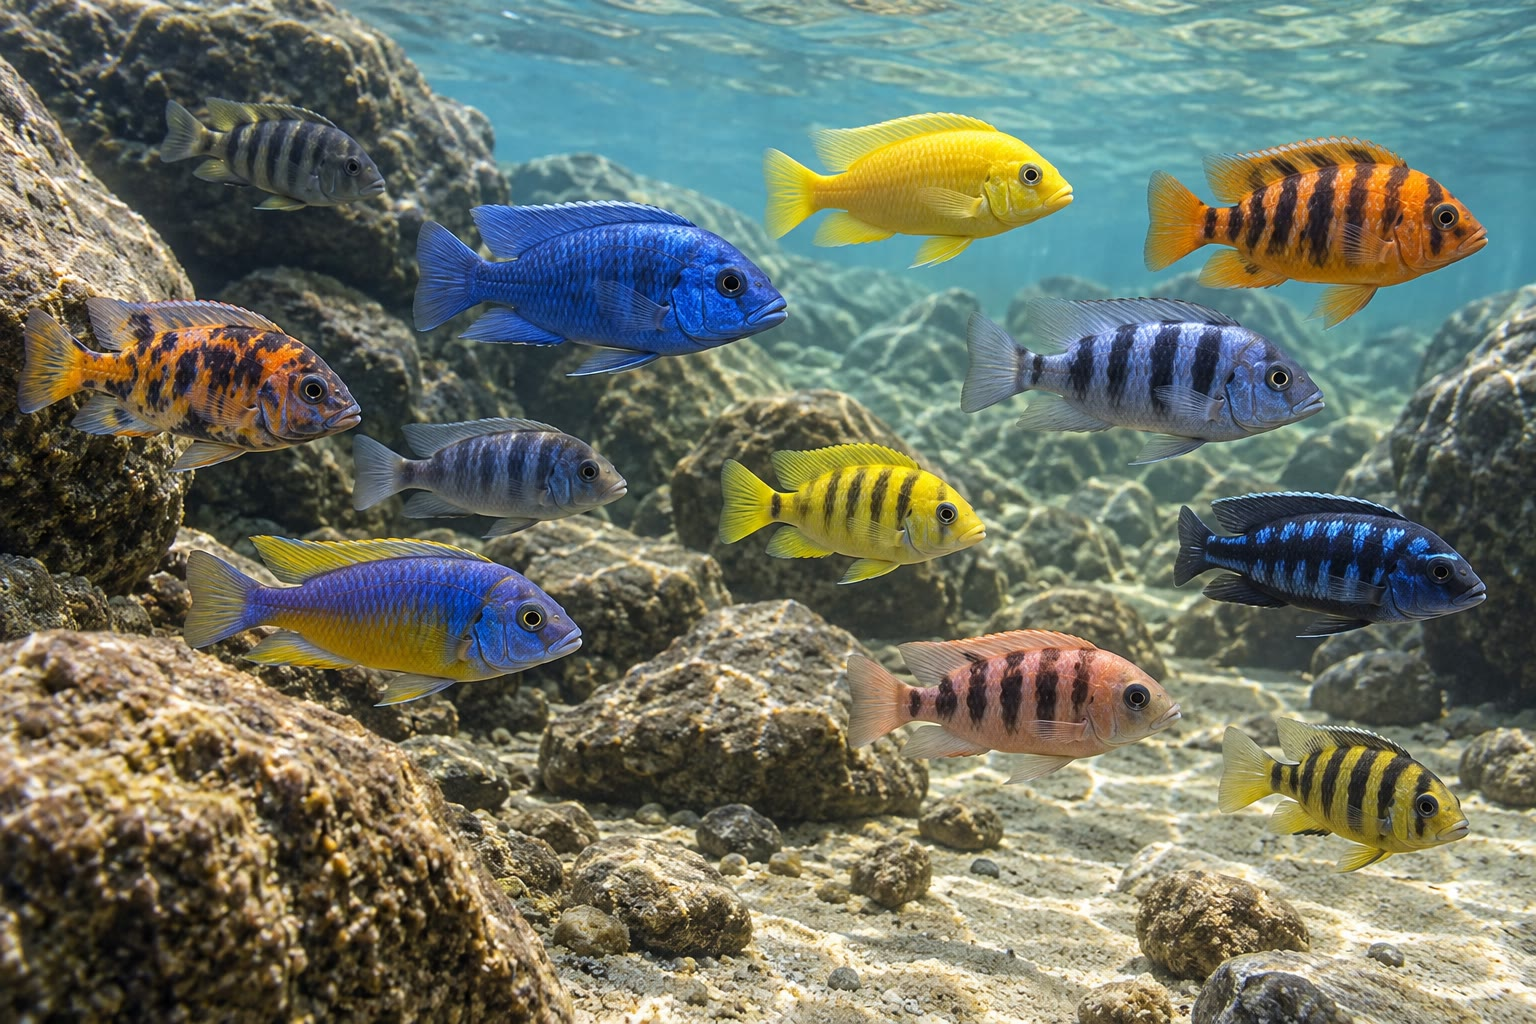
\includegraphics[width=0.6\linewidth]{images/book5/ai/b5-25-cichlids.jpg}

{\small 非洲某湖的丽鱼：数百个物种
在数千年间形成，其差异主要源于
其共同祖先早已携带的变异。}
\end{omfigure}

\begin{remark}[以偶然性为基线]\label{rem:b3:molecular-evolution:remark}
\omterm{thm:b3:molecular-evolution:neutral}{中性理论}并非断言选择不重要；它
陈述的是选择缺失时会发生什么，其表述足够精确，
足以被检验。由于中性速率即突变速率，
分化程度可以度量时间；由于中性变化填满了
选择留下的空位，$\omega$ 度量约束；由于中性
谱系以已知速率合并，\omterm{prop:b3:molecular-evolution:ils}{基因树}的不一致
度量了无人见过的种群大小。选择便是
扣除偶然性之后所剩下的部分——例如 $\omega$ 大于
一的基因、一次清除某区域变异的选择扫荡，以及一棵
分歧方向漂变无法解释的树。南极冰鱼的
抗冻蛋白、反刍动物的胃溶菌酶，以及灵长类的第三种视蛋白
是以这种方式发现的例外，每一个都讲述了一个基因被复制并获得
新功能的故事。基因组的其余部分则是一只\omterm{prop:b3:molecular-evolution:clock}{分子钟}。
\end{remark}

\section{练习}

\begin{exercise}[$\star$]\label{exo:b3:molecular-evolution:1}
写出中性\omterm{thm:b3:molecular-evolution:neutral}{替换速率}，并用文字解释它为何
不依赖种群大小。
\end{exercise}

\begin{exercise}[$\star$]\label{exo:b3:molecular-evolution:2}
定义\omterm{def:b3:genomics:comparative}{直系同源基因}、\omterm{def:b3:genomics:comparative}{旁系同源基因}和\omterm{def:b3:molecular-evolution:duplication}{假基因}，各举一例，
取自珠蛋白家族。
\end{exercise}

\begin{exercise}[$\star$]\label{exo:b3:molecular-evolution:3}
$\omega = d_{N}/d_{S}$ 度量什么？解释 $\omega = 0.02$，
$\omega = 1.0$ 和 $\omega = 2.5$ 的含义，并各举一个此类基因。
\end{exercise}

\begin{exercise}[$\star$]\label{exo:b3:molecular-evolution:4}
木村资生为何断定多数替换是中性的？请用本章开头
的数据重述这一论证。
\end{exercise}

\begin{exercise}[$\star\star$]\label{exo:b3:molecular-evolution:5}
$N = 5000$。计算新突变在 $s
= 0$、$s = 0.001$、$s = 0.01$ 和 $s = -0.001$ 下的\omterm{thm:b3:molecular-evolution:neutral}{固定概率}（用木村资生公式），
并讨论其中哪些实际上可视为中性。
\end{exercise}

\begin{exercise}[$\star\star$]\label{exo:b3:molecular-evolution:6}
两个物种在某基因的 \qty{12}{\%} 位点上存在差异，该基因的中性
速率为每位点每年 \qty{2e-9}{}。估计二者的分歧时间，
分别在使用和不使用朱克斯–康托尔校正的情况下计算。原始差异为多少时，
校正使估计值达到原始值的两倍？
\end{exercise}

\begin{exercise}[$\star\star$]\label{exo:b3:molecular-evolution:7}
一个基因含 300 个密码子，有 700 个非同义位点和 200 个同义位点。
两个物种之间，该基因显示 7 个非同义差异和 10 个同义
差异。计算（未校正的）$p_{N}$、$p_{S}$ 和 $\omega$。属于哪种
选择模式？若计数改为 35 和 10，结果如何？
\end{exercise}

\begin{exercise}[$\star\star$]\label{exo:b3:molecular-evolution:8}
人和黑猩猩的中性序列在 \qty{1.2}{\%} 的位点上存在差异；
分化发生在 \qty{6.5}{Myr} 前，世代时间为 \qty{25}{yr}。估计
每位点每代的突变率，以及
每代在含 $6\times 10^{9}$ 个碱基的二倍体基因组中产生的新突变数。
\end{exercise}

\begin{exercise}[$\star\star$]\label{exo:b3:molecular-evolution:9}
取 $N = \num{50000}$，两次分化之间相隔 $T = \num{100000}$ 代，
计算\omterm{prop:b3:molecular-evolution:ils}{基因树}与\omterm{prop:b3:molecular-evolution:ils}{物种树}不一致的比例，
分别对人、黑猩猩和大猩猩计算。何种 $T$ 会使该比例达到
\qty{10}{\%}？
\end{exercise}

\begin{exercise}[$\star\star\star$]\label{exo:b3:molecular-evolution:10}
证明木村资生公式的极限为 $1/2N$（$s \to 0$ 时），趋于 $2s$ 的条件
为 $4Ns \gg 1$；并证明当 $s < 0$ 且 $4N|s| \gg 1$ 时，其行为近似为
$2|s|\,\mathrm{e}^{-4N|s|}$。由此估计，一个突变须有多强的有害性，
才能使其在大小为 $10^{4}$ 的种群中的\omterm{thm:b3:molecular-evolution:neutral}{固定概率}
较中性情形降低百倍。
\end{exercise}

\begin{exercise}[$\star\star\star$]\label{exo:b3:molecular-evolution:11}
相对速率检验：外群 $O$ 与小鼠的校正距离为 $0.30$，
与人的为 $0.24$，小鼠与人相距 $0.20$。计算小鼠与人自分歧以来的
分支长度（假设分歧点到
$O$ 的两条路径等长），以及二者的比值。小鼠世代为
\qty{0.5}{yr}，人为 \qty{25}{yr}。若采用严格的每世代
\omterm{prop:b3:molecular-evolution:clock}{分子钟}，比值应为多少？这一
观测对每代突变率说明了什么？
\end{exercise}

\begin{exercise}[$\star\star\star$]\label{exo:b3:molecular-evolution:12}
一个复制基因解除了约束（$\omega = 1$），
以中性速率 $k = \qty{2e-9}{}$ 每位点每年演化。在一个 1000
碱基的编码序列中，预期需要多少年才会首次出现终止密码子或
移码？（假设约 \qty{4}{\%} 的随机点突变
会在编码序列中产生终止密码子，并忽略插入缺失）？
将其与选择发现新功能所需的时间相比较，并解释
为何多数复制基因会消亡。
\end{exercise}

\section{问题：变化速率}

\begin{problem}[{周末问题——以数字写就的基因组历史：
由人与黑猩猩分歧推算突变率，木村资生
替换负荷，被选择突变的固定概率，基因的
$\omega$ 由密码子计数得到，复制基因的分子钟读数，并
类人猿之间基因树的不一致，以突变率为终，
该基因的 $\omega$ 与不一致比例}]
\label{pb:b3:molecular-evolution:1}
数据：人与黑猩猩的中性分歧 $d = 0.012$；分化
\qty{6.5}{Myr} 前；世代 \qty{25}{yr}；二倍体基因组 $6\times
10^{9}$ 个碱基，其中 \qty{1.5}{\%} 为编码区。祖先种群 $N =
\num{50000}$。基因：400 个密码子，920 个非同义位点、280 个同义
位点；人与小鼠的差异为 46 个非同义、84 个同义。
人与小鼠的分化发生于 \qty{90}{Myr} 前。珠蛋白：$\alpha$ 与 $\beta$ 在
\qty{55}{\%} 的氨基酸位点上存在差异（未校正）；血红蛋白速率为 \num{1e-9}
每位点每年。类人猿：大猩猩与黑猩猩两次分化之间的 $T$
为 \num{80000} 代。霍尔丹极限：每
300 代一次被选择的替换。

\medskip
\noindent\textbf{第一部分——速率。}
\begin{enumerate}
  \item 由 $d = 2kT$ 计算每位点每年的 $k$，进而求每
        位点每代的 $\mu$。
  \item 每代每个二倍体基因组的新突变数，以及其中
        有多少落在编码序列中。
  \item 按中性速率计，全基因组每代固定的替换数
        （种群每位点每代固定 $\mu$），
        与霍尔丹极限比较，并得出木村资生的
        结论。
  \item 在 $N = \num{50000}$ 的种群中，全种群每代每位点
        会新产生多少中性突变，
        其中多大比例最终会固定？
  \item 注定会固定的中性突变需要多长时间？请分别以代数和
        年计，并与自人与黑猩猩
        分化以来的时间相比较。
  \item 解释为何尽管有第~5~小题的结论，两个物种之间的分歧
        度量的是自二者分化以来的时间，而不是
        自其等位基因固定以来的时间。
\end{enumerate}

\medskip
\noindent\textbf{第二部分——选择的概率。}
\begin{enumerate}[resume]
  \item 中性突变在 $N = \num{50000}$ 时的\omterm{thm:b3:molecular-evolution:neutral}{固定概率}，
        以及 $s = 0.001$、$s = 0.01$、$s = 0.1$ 的突变的\omterm{thm:b3:molecular-evolution:neutral}{固定概率}。
  \item 对于哪些 $s$ 满足 $4Ns = 1$？解释这一临界情形的含义。
  \item 有害突变（$s = -0.001$）的\omterm{thm:b3:molecular-evolution:neutral}{固定概率}，
        与中性突变相比为多少？$s = -10^{-5}$ 时又如何？
  \item 若某基因的新突变中，比例为 $10^{-5}$ 的突变有益，
        $s = 0.01$，其余为中性突变，则该基因替换中的适应性替换占多大比例？
        并评论：即使选择确实在起作用，
        它在序列中也很少显现出来。
  \item 计算人–小鼠该基因的 $p_{N}$ 和 $p_{S}$，
        分别用 Jukes--康托尔方法校正，并给出 $\omega$。
  \item 解释 $\omega$；并估计该基因的中性速率，
        由 $d_{S}$ 推出（每位点每年），利用分化时间计算。这是否
        与第~1~问相符？
\end{enumerate}

\medskip
\noindent\textbf{第三部分——时钟与副本。}
\begin{enumerate}[resume]
  \item 对 $\alpha$--$\beta$ 珠蛋白的差异进行多重
        替换校正（采用 $d = -\ln(1 - p)$，即允许多状态的蛋白质版本），
        并用血红蛋白速率确定该次复制的时间。
  \item 该时间接近有颌脊椎动物的起源
        （\qtyrange{450}{500}{Myr}）。拥有独立的 $\alpha$
        和 $\beta$ 链，能实现哪些单链做不到的事？
  \item 纤维蛋白肽以每位点每年 $8\times 10^{-9}$ 的速率变化。
        两个物种于 \qty{40}{Myr} 前分化，预期原始差异为多少？
        为何该蛋白质无法用于
        对 \qty{500}{Myr} 的分化进行定年？
  \item \omterm{def:b3:chromatin-epigenetics:nucleosome}{组蛋白} H4 以 $10^{-11}$ 的速率变化：在 100 个位点上，
        经过 \qty{1000}{Myr} 会发生多少次替换？为何它不适用于
        对近期的分化进行定年？
  \item 一个副本基因自复制时刻起以 $\omega = 1$ 漂变，
        若编码序列中 \qty{4}{\%} 的替换产生终止密码子，
        且该基因有 1200 个位点，速率为 $2\times
        10^{-9}$ 每位点每年，估计期望的
        首个终止密码子出现时间。
  \item 为何\omterm{def:b3:genomics:comparative}{全基因组复制}比单次串联复制使副本
        具有更好的存活机会？
\end{enumerate}

\medskip
\noindent\textbf{第四部分——树中之树。}
\begin{enumerate}[resume]
  \item 人与黑猩猩谱系未能合并的概率，
        即在大猩猩分化前的 \num{80000} 代内未发生合并。
  \item 与\omterm{prop:b3:molecular-evolution:ils}{物种树}不一致的\omterm{prop:b3:molecular-evolution:ils}{基因树}所占比例。
        观测值约为 \qty{30}{\%}。是否相符？
  \item 在不一致的\omterm{prop:b3:molecular-evolution:ils}{基因树}中，人与大猩猩聚为一类的比例为多少，
        黑猩猩与大猩猩聚为一类的比例又是多少？若两者显著偏离相等，
        将说明什么？
  \item 若祖先种群为 $N = \num{10000}$，
        预期的不一致比例应为多少？观测到的
        比例因此说明我们祖先的种群数量如何？
  \item 将一千个基因拼接为一个\omterm{def:b3:bioinformatics:alignment}{比对}，为何会得到
        一棵置信度很高但可能错误的树，而溯祖方法则
        改为怎样做？
  \item 非洲以外人群中的尼安德特人 DNA 约占 \qty{2}{\%}，
        携带该片段的树中，部分欧洲人与尼安德特人聚为一类的频率
        高于非洲人。为何这不是\omterm{prop:b3:molecular-evolution:ils}{不完全谱系分选}？
  \item 总结：$\mu$（第~1~问）、该基因的 $\omega$
        （第~11~问）以及不一致比例（第~20~问）。
\end{enumerate}
\end{problem}
